\chapter{Formas de Validações das Novas Abstrações de Processos}
\label{cap:validacoes}

O Capítulo \ref{cap:trabalhos-analisados} mostrou algumas das pesquisas que
buscam estender a abstração de processos atual. Apesar de vários trabalhos
demonstrarem algum tipo de benefício, muitos deles ignoram outros aspectos. Por
exemplo, uma abordagem que visa isolar dados para evitar vazamento de
informações faz testes que buscam tal falha, mas não valida se a alteração é
viável em um contexto global com alta demanda.  Adicionalmente, alguns desses
trabalhos se baseiam fortemente em \textit{microbenchmarks} o que claramente
pode evidenciar um resultado desejado e não explicitar um efeito colateral da
alteração. Em busca de encontrar propostas de abstrações que podem ser levada
para os SO atuais e também beneficiar aplicações no espaço do usuário,
levantamos e respondemos as seguintes perguntas:

\begin{quote}
 \item \textit{RQ3:.} "Quais aplicações podem ser utilizadas para avaliar as nova abstração adicionadas ao SO?"
 \item \textit{RQ4:.} "Qual conjunto de \emph{microbenchmark} pode ser utilizado para auxiliar a entender os impactos de uma nova característica adicionada para as abstrações de processos?"
\end{quote}

Defendemos que uma das formas mais eficientes para validar uma nova extensão da
abstração é por meio de aplicações já consagradas, amplamente adotadas por
diversos sistemas e que exercitam uma ou mais parte do SO. Por esses motivos
buscamos por algumas aplicações que auxiliam a demonstrar que uma proposta é
valida ou não. Basicamente buscamos três características: estresse que a
aplicação pode gerar, possíveis falhas de segurança e mecanismos periféricos.
Aplicações que consomem muitos recursos de hardware são ideais para comprovar
que uma nova extensão é escalável. Por outro lado, várias propostas de novos
mecanismos no processo prometem melhorias de segurança, por esse motivo
software reais que já apresentaram alguma falha de segurança são desejáveis
para esse tipo de validações. Por fim, algumas pesquisas propõem novos
mecanismos nos quais alguns tipos de aplicações podem se beneficiar, como por
exemplo, o compartilhamento de memória e otimizações.

Outra perspectivas sobre a validação que merece atenção é o uso de
\textit{microbenchmarks} que auxiliam no estudo dos impactos das alterações.
Tais testes, são vantajosos durante as etapas iniciais da nova abstração uma
vez que são rápidos e ajudam durante o desenvolvimento. O conjunto de
\textit{microbenchmarks} pode ser usado para indicar de que a nova abstração
traz vantagens, contudo, dado o seu alto grau de isolamento esse não consegue
revelar a real natureza de uma alteração.

A analise feita sobre as aplicações e \textit{microbenchmarks} tiveram como
origem os diversos experimentos realizados pelos pesquisadores que mostramos no
Capítulo \ref{cap:trabalhos-analisados}. Além disso, durante esse trabalho,
foram conduzidos experimentos que auxiliaram na construção desse capítulo.

\section{Servidores Web}

%TODO: Lembrar de adicionar alguns conceitos apresentados aqui no index

Normalmente um software faz uso de diversos recursos do SO, contudo, algumas
aplicações são projetadas para tirar o maior proveito possível do hardware
disponível. Muitos sistemas possuem máquinas dedicadas com o objetivo de
entregar estabilidade, velocidade e estabilidade. Nesses casos, é desejável que
a CPU esteja ocupada a maior parte do tempo e use a memória de forma eficiente
para evitar desperdício de recursos. \boldAndIndex{Servidores web (\textit{Web
Servers)}} são um tipo de aplicação que tenta operar com um desempenho próximo
do ótimo utilizando ostensivamente os recursos das máquinas para servir páginas
webs. A principal responsabilidade do servidor web é entregar arquivos contendo
dados, por sua vez essa tarefa pode ser divida em três: esperar por uma
requisição (\textit{request}) do usuário, processar a requisição e responder ao
usuário.

\begin{figure}[!h]
  \centering
  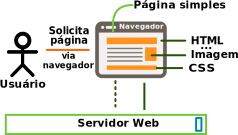
\includegraphics[width=.60\textwidth]{request_a_page.png}
  \caption{Do cliente para o servidor Web}
  \label{fig:client_to_web_server}
\end{figure}

A Figura \ref{fig:client_to_web_server} busca exemplificar uma situação simples
na qual o cliente solicita uma página web para um servidor. Primeiramente, o
cliente faz uma solicitação de alguma página por meio de algum software, para
esse exemplo vamos considerar o navegador. Em seguida o navegador comunica-se
com o servidor utilizando o protocolo HTTP que por sua vez devolve um arquivo
contento todas as instruções básicas necessárias para construir a página
(normalmente um arquivo HTML). O navegador abre o arquivo HTML retornado,
converte o conteúdo e verifica se precisa de mais informações para construir a
página solicitada; é comum que a página precise de outros arquivos como CSS,
imagens, javascript, etc. Se mais arquivos forem necessários, então o navegador
solicita os mesmos para o servidor de forma paralela ou serial. O exemplo
ilustra de forma simplificado como uma requisição acontece e como múltiplas
requisições podem ser geradas para construir uma simples telas. Com um exemplo
real, uma caracterização da carga gerada para o site da copa do mundo de 1998
mostra que 10796 requisições/min foram feita para o cite \citep{worldcup}. Um
servidor web tem que responder milhares de usuários e a estrategia utilizada
para lidar com tal problema são as mais variáveis possível.

\begin{figure}[!h]
  \centering
  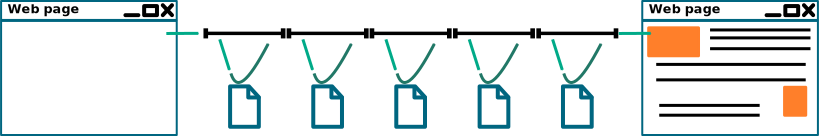
\includegraphics[width=\textwidth]{no_keep_alive.png}
  \caption{Sem keep alive}
  \label{fig:no_keep_alive}
\end{figure}

\begin{figure}[!h]
  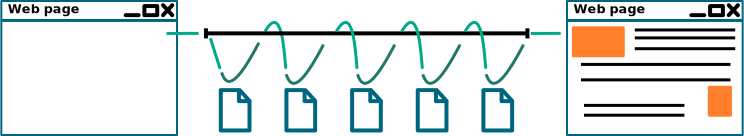
\includegraphics[width=\textwidth]{keep_alive.png}
  \caption{Com keep alive}
  \label{fig:keep_alive}
\end{figure}

Normalmente, cada requisição feita por um cliente abre muitas conexões com o
servidor web e ao final de cada uma é feito o encerramento da conexão. Esse
mecanismo impacta no desempenho por duas razões: a latência aumenta e o consumo
de CPU com operações não uteis se eleva. Uma possibilidade para minimizar esses
impactos é utilizar um mecanismo chamado de \boldAndIndex{keep-alive} que
fornece uma conexão aberta durante as atividades dos usuários. Por exemplo, a
Figura \ref{fig:no_keep_alive} e a Figura \ref{fig:keep_alive} mostram um caso
utilizando \textit{keep-alive} e outra sem utilizar. O primeiro caso mostra a
situação na qual uma requisição é feita por um cliente, por sua vez é aberto
uma nova conexão que é mantida aberta. Em geral, o \textit{keep-alive} reduz a
latência e o uso de CPU no servidor web o que pode melhorar a experiência do
usuário no caso de um servidor que esteja recebendo um elevado número de
requisições. Contudo, outro aspecto do \textit{keep-alive} é que esse pode
elevar o consumo de memória o que é um problema em um servidor sobrecarregado.

Existem muitos servidores web disponíveis no mercado, contudo dois deles são
especialmente relevantes para o contexto desse trabalho: Nginx e Apache Httpd.
O primeiro é conhecido pelo seu desempenho para entregar arquivos estáticos,
enquanto o segundo é conhecido pela sua enorme estabilidade e extensões. Ambos
são extremamente configuráveis, confiáveis e suportam grandes cargas de
requisições.

\subsection{Servidor Apache HTTP}
\label{sec:architecture}

O servidor Apache HTTP, também conhecido como \textit{HTTP Daemon (HTTPD)} é
licenciado com a licença Apache 2.0 e mantido pela fundação Apache.  O Apache
HTTP (usaremos HTTPD e Apache como sinônimos nesse texto) foi projetado para
executar em vários SOs, essa restrição fez com que fosse necessário adotar
estratégias para fazer o HTTPD multiplataforma e sem perder desempenho. Por
esse motivo o Apache é fortemente modularizado, utiliza bibliotecas portáveis e
separa os módulos de manipulação de processos e threads; esse três elementos
constituem os pilares arquiteturais do projeto. O núcleo do HTTPD tem apenas
alguns elementos, contudo o conjunto de todos os módulos usados pelo servidor
faz com que ele seja modularizado e flexível. O Apache também utiliza a
biblioteca \textit{Apache Portable Runtime (APR)} cujo intenção é servir como
uma interface portável para as tarefas comuns de programação (e.g.: alocação de
memória, manipulação de tempo, etc). Por fim, o HTTPD implementa um módulo
especial chamado de \textit{Multi-Processing Module (MPM)} que é responsável
por manter o processamento das requisições e a lógica de manipulação de
processos/threads. O MPM representa uma rica fonte para comparar modificações
nas abstrações de processos.

\begin{figure}[!h]
  \centering
  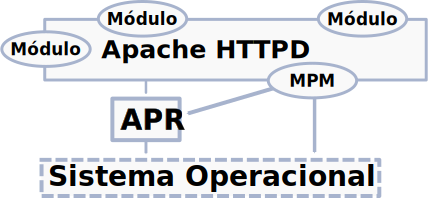
\includegraphics[width=.7\textwidth]{apache_arhitecture} 
  \caption{Arquitetura do servidor Apache HTTP \citep{apache_module_book}}
  \label{fig:apache_architecture} 
\end{figure}

A Figura \ref{fig:apache_architecture} é uma visão de alto nível da arquitetura
do Apache. O centro da imagem representa os elementos do núcleo do Apache que
são responsáveis por juntar os demais componentes necessários para o seu
funcionamento. Ao redor do núcleo, existe um grande número de módulos anexados
que podem ser conectados ao projeto. Esses módulos facilitam o processo de
adicionar e remover elementos ao núcleo, normalmente esses componentes são
ligado como bibliotecas dinâmicas (também podem ser estáticas). Módulos na
forma de biblioteca lincadas dinamicamente fornecem flexibilidade, um bom
desempenho e portabilidade entre diferentes SOs (e.g.; o Window e Linux podem
ter diferentes implementações para o mesmo módulo). A Figura
\ref{fig:apache_architecture} também ilustra o MPM como um componente
diretamente conectado ao SO, porque o MPM manipula os elementos de
paralelização e cada SO precisa implementar essa parde de acordo com a suas
próprias particularidades. A última parte da imagem, mostra a biblioteca APR
que se posiciona entre o núcleo do HTTPD e o SO.

\begin{figure}[!h]
  \centering
  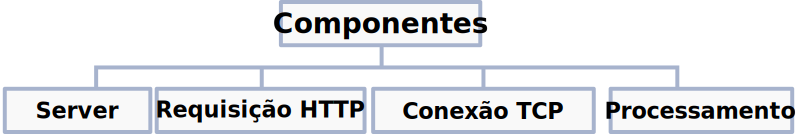
\includegraphics[width=.7\textwidth]{units} 
  \caption{Unidade do Servidor Apache HTTP}
  \label{fig:units} 
\end{figure}

Alguns módulos são essenciais para o funcionamento do HTTPD uma vez que eles
representam os elementos básicos das estruturas de dados que são usadas por
todo o código. A Figura \ref{fig:units} mostra algumas unidade fundamentais
usadas pelo HTTPD. O módulo "server" é responsável por criar uma estrutura de
dados para a requisição toda vez que o HTTPD aceita uma nova conexão. O módulo
HTTP é responsável por preencher uma estrutura de dados de requisição e o
módulo de conexão TCP constrói a estrutura de dados que mantém as informações
da conexão. Normalmente, não é preciso se preocupar com módulos relacionados
aos detalhes do HTTP uma vez que o Apache ajusta todos os elementos necessários
e também entrega uma estrutura de dados pronta para ser utilizadas.

\begin{figure}[!h]
  \centering
  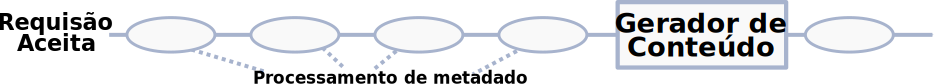
\includegraphics[width=.9\textwidth]{request_phases} 
  \caption{Gerador de Conteúdo \citep{apache_module_book}}
  \label{fig:content_generator} 
\end{figure}

O último aspecto importante da arquitetura do Apache é o \textbf{Content
Generator} (Gerador de Conteúdo), este funciona como uma linha de produção da
resposta HTTP \citep{apache_module_book}. Para cada requisição feita para o
HTTPD, ele cria um \textit{Content Generator}; esse pode ser customizado com
algum outro módulo que faz operações intermediárias (e.g.: adicionar um campo
extra na construção do resposta). A Figura \ref{fig:content_generator} mostra
as fases padrão, repare que depois que uma requisição é aceita o HTTPD realiza
diversos passos até que a resposta seja construída. Embora a maioria dos casos
se encaixam no caso padrão outras situações podem demandar fases adicionais,
princípalmente para testes em novas abstrações de processos.

\subsubsection{MPM}

O módulo \textit{Multi-Processing (MPM)} é um elemento especial dentro do HTTPD. Com a Seção \ref{sec:architecture} introduziu, ela funciona como uma interface entre o HTTPD e o SO. O MPM tem três características princípais para qualquer instância do Apache: único, obrigatório e tem uma implementação específica. O HTTPD fornece pelo menos um módulo MPM por SO (segurança e desempenho), por exemplo, o Window utiliza \texttt{mpm\_winnt} e o Linux tem três opções diferentes.

Cada uma das três opções podem ser classificadas como baseada em processos ou em threads, mais epecificamente são elas: \textit{Prefork}, \textit{Worker} e \textit{Event}. Esses módulos podem ser grandes elementos para comparar thread e processos usando as novas abstrações.

\subsubsection{MPM: Prefork}
\label{sec:prefork}

\begin{figure}[!h]
  \centering
  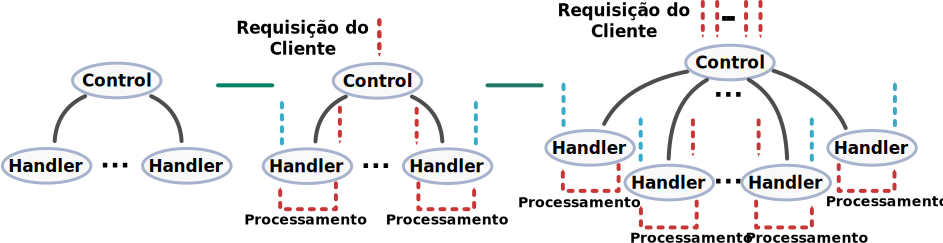
\includegraphics[width=\textwidth]{prefork} 
  \caption{Prefork}
  \label{fig:prefork} 
\end{figure}

O \textit{Prefork} foi a primeira estratégia adotada pelo HTTPD que é totalmente baseado em processos. O HTTPD inicia com um processo responsável por gerir processos filhos que serão manipulados por uma única requisição. A Figura \ref{fig:prefork} ilustra os três passos realizados pelo \textit{Prefork}. Primeiramente o HTTPD incia com um único processo responsável por realizar o controle das tarefas e alguns processos filhos prontos para atender a qualquer requisição. Em seguida, se alguma requisição chegar o controle é passado para o processo responsável por passar a tarefa de manipular a solicitação para um processo que esteja sem fazer nada. Por fim, se não existir nenhum processo filho disponível, o processo de controle cria vários processos filhos novos.

O \textit{Prefork} é uma boa opção para servidores web que não são compatíveis com threads (e.g. aplicações legadas em PHP) e é a melhor opção de MPM para isolar uma única requisição. Contudo, o \textit{Prefork} consome muita memória e CPU o que não é desejável em um servidor sob forte demanda.

\subsubsection{MPM: Worker}

O \textit{Worker} é uma solução híbrida uma vez que o seu design é baseado em processos e threads. Esse módulo tem um processo de control que é responsável por crear um processo filho e balancear a carga. Ao contrário do \textit{Prefork} o Worker não cria instâncias de processos filhos para manipular requisições dos clientes. Ele cria diversas processos novos com várias threads para realizar essa tarefa, ocasionalmente, o HTTPD tem que manipular um grande número de requsições e nesse caso o controle de processo atua criando um grande número de filhos (cada um com um grande conjunto de threads) para suportar a carga. Repare que o \textit{Worker} utiliza threads para manipular requisições que decressem o total de processos filhos (comparado com o \textit{Prefork}) e o consumo de memória. O HTTPD tem um arquivo de configuração que permite um controle fino de todos os parametros relacionados ao número máximo de processos filhos, o total de threads por filhos, o número de reposição de processos fihos e threads, dentre outros.

\begin{figure}[!h]
  \centering
  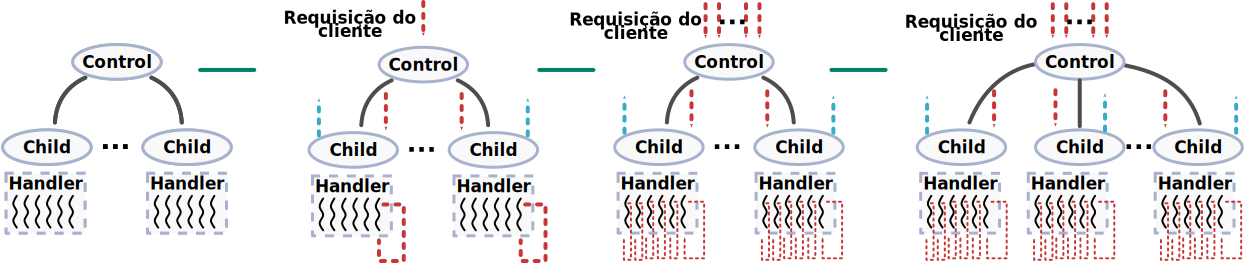
\includegraphics[width=\textwidth]{worker} 
  \caption{Worker}
  \label{fig:worker} 
\end{figure}

A Figura \ref{fig:worker} é um exemplo de como o \textit{Worker} funciona. Quando o HTTPD inicia, ele tem um processo de controle em adição a alguns processos filhos que mantém um grupo de threads paradas. A segunda parte da figura representa o cado em que o HTTPD recebe um grande número de requisições e o processo de controle cria mais filhos para suportar a carga. O \textit{Worker} consome muito menos memória que o \textit{Prefork} e consequentemente ele é melhor em casos no qual o servidor está sobrecarregado. A mistura de processo e thread adiciona estabilitade para todo o sistema.

\subsubsection{MPM: Event}

\begin{figure}[!h]
  \centering
  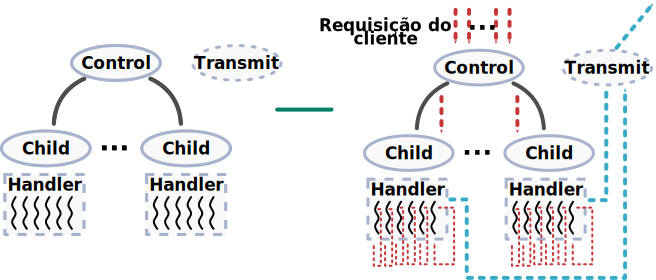
\includegraphics[width=.7\textwidth]{event} 
  \caption{Event}
  \label{fig:event} 
\end{figure}

O módulo \textit{Event} é baseado em threads e é o padrão na última versão do Apache. O comportamento básico do \textit{Event} é similar ao do \textit{Worker} com duas características princípais: \textit{keep-alive} e separação de responsábilidade para enviar dados para o cliente. A Figura \ref{fig:event} ilustra o comportamento básico do \textit{Event}. Os passos são similares ao do \textit{Worker} com um processo extra manipulando o transmissão dos dados. Então a requisição processada passa o resultado final para a thread responsável por enviar o resultado para o cliente.

\subsection{Nginx}

Assim ocmo o Apache Httpdd o Nginx é um servidor web, contudo esse diferencia-se de muitas formas dos servidores web tradicionais. A sua princípal característica é o seu elevado desempenho para atender requisições, principlamente aquelas relacionadas a arquivos estáticos. Além disso o Nginx comporta-se como um reverse-proxy; ele recebe uma requisição do usuário, por sua vez ele repassa para uma aplicação especifica. Quando o dado é processado pela aplicação, essa retorna o resultado para o Nginx que repassa os dados para o usuário \citep{soni}. A Figura X ilustra o caso explicado e uma segunda variação na qual uma operação intermediária pode ser inserida (no exemplo, o SSL).

% TODO: Figura X

A grande maioria dos servidores web buscam tirar o máximo proveito dos recursos de hardware utilizando um elevado número de threads e processos. Essa abordagem é relativamente simles de ser implementada e traz bons resultados, contudo ela também tem alguns problemas. Dentre as desvantagens, temos que o modelo baseado em threads/processos geram uma grande quantidade de operações que bloqueiam e consequentemente geram trocas de contexto. Além disto, a abordagem baseada em threads/processos consome uma elevada quantidade de recursos o que por sua vez degrada o desempenho da aplicação.

O Nginx sugere uma abordagem nova para os problemas referentes ao servidor web, que se baseia em evento. A estratégia aborda parte do princípio que deve-se evitar ao máximo a troca de contexto e deve-se utilizar ao máxmo a CPU com processamento útil. Por esse motivo o Nginx cria três tipos de processos \citep{nginx_architecture}:

\begin{itemize}
  \item Processo master, faz operações privilégiadas como ler arquivos de configuração e acessar portas;
  \item Processo que faz cache carregando dados do disco fazendo cache na memória;
  \item Processo que gerencia o cache verificando o mesmo periodicamente;
  \item Processos \textit{Worker} são os processos que fazem o trabalho de manipular conexões, ler e escrever em disco e comunicar-se com os servidores.
\end{itemize}

O Nginx recomenda um \textit{Worker} por núcleo da CPU, isso permite tirar grande proveito dos eventos.

Na prática o sistema de eventos é eficiênte pois nã gera bloqueios uma vez que esse não espera a aplicação terminar o que está fazendo. Por exemplo, se o \textit{worker} estiver atendendo uma requisição e em determinado momento precisar recuperar uma informação do disco o \textit{worker} não bloqueia, ele simplesmente vai fazer outra tarefa. O sistema de eventos faz com que um único \textit{worker} execute multiplas tarefas de forma sequêncial sem bloqueio e consequentemente com poucas trocas de contexto.

\section{Ferramentas de comunicação encriptada}

%TODO: Além da introdução, vale uma explicação sobre CVE

\subsection{OpenSSL}

Antes de tratar sobre o OpenSSL é imortante apresentar de forma geral o protocolo \textit{Secure Sockets Layers (SSL)}. O princípal objetivo do SSL é fornecer um conjunto de protocolos criptográficos que permita a comunicação segura na rede. Basicamente, esse constituí uma ferramenta de uso codiano, tendo diversas aplicações de missão crítica dependendo de tal protocolo o que faz dele um constante alvo de ataques.

O SSL e outros possuem um mecanismo chamado de \textit{handshake} que nada mais é do que um processo de negóciação entre cliente e servidor de forma a criar a conexão segura entre ambos, a Figura \ref{fig:openssl_handshake} descrever de forma geral os passos da negóciação. O processo de negociação começa com o cliente mandando uma mensagem de "Oi, do cliente" para o servidor, nela o cliente informa a versão do SSL que está usando, os algoritmos de criptografia e os métodos de compressão. O servidor por sua vez manda um "Oi, vindo do servidor" dizendo qual algoritmo usar (selecionado da lista que o cliente mandou), um ID da seção, um certificado digital e a sua chave pública.Com o certificado, o cliente consulta uma "Certificate Authority (CA)" que valiad se o servidor é valido ou não, isso serve para estabelecer a confiança. Depois que o cliente acredita no seridor, começa a etapa de troca de chaves na qual o cliente envia a chave secreta compartilhável com a chave pública do servidor (o cliente termina enviando uma mensagem de fim). O servidor descripta a mensagem do cliente e utiliza a chave enviada para criptografar uma mensagem de fim e envia para o cliente. Quando o \textit{handshake} termina, o servidor e o cliente podem enviar mensagens que são siméticamente encriptadas \citep{openssl}.

\begin{figure}[!h]
  \centering
  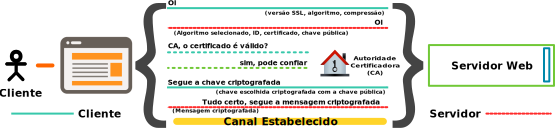
\includegraphics[width=\textwidth]{ssl_handshake}
  \caption{Do cliente para o servidor Web}
  \label{fig:openssl_handshake}
\end{figure}

O OpenSSL é uma implementação livre do protocolo SSL, ele contém a implementação de várias funções criptográficas e funçõs utilitárias. A Figura \ref{fig:openssl_arch} mostra uma visão geral da arquitetura do OpenSSL. O \textit{EVP crypto API} são funções de alto nível que fornecem recursos para derivação de chaves, hash seguro, código de autenticação de mensagens, encriptação/decriptação de algoritmos simétricos/assimétricos, dentre outros. A arquitutra também fornece uma pilha de manipulação de erros e uma interface abstrada para lidar com I/O.


\begin{figure}[!h]
  \centering
  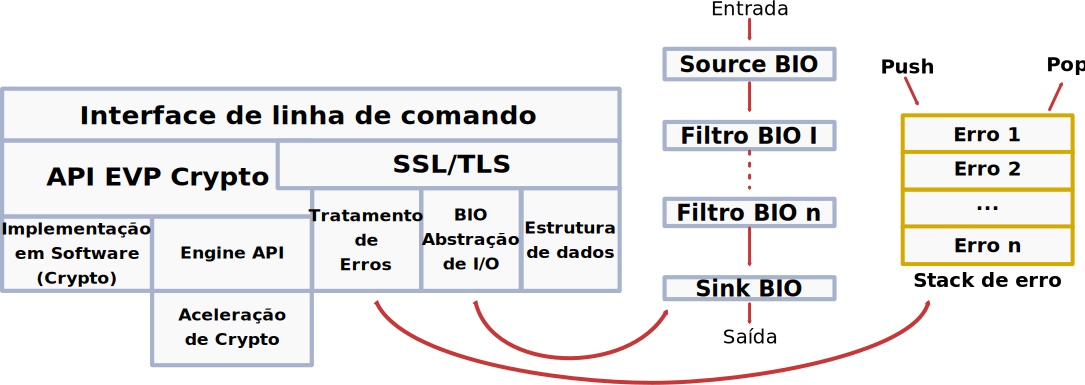
\includegraphics[width=\textwidth]{openssl_arch}
  \caption{Do cliente para o servidor Web \citep{crypto_openssl}}
  \label{fig:openssl_arch}
\end{figure}


\subsection{OpenSSH}

Hoje em dia, uma das tarefas mais comuns do dia-a-dia de muitos desenvolvedores consiste em acessar servidores em diversos locais do mundo e configurar uma determinada aplicação. Na prática, boa parte dos profissionais de TI faz uso de conexões seguras na Internet por meio do protocolo \textit{Secure Shell (SSH)}. Existem diversas implementações deste protocolo, discutiremos aqui de forma breve o OpenSSH.

A Figura \ref{fig:openssh_layer} apresenta uma visão geral da arquitetura do OpenSSH. Primeiramente repare que as três camadas correspondentes as camadas SSH encontram-se sobre a camada TCP/IP que consistem em uma conexão nã segura. Aprimeira camada se chama \textit{ssh-transport} e ela é responsável por realizar operações criptográficas, proteção contra atques e reverificar chaves de temos em tempos. Logo após a primeira camada temos o \textit{ssh-userauth} que é responsável pela autenticação, se tudo der certo durante a autenticação então a troca de chaves acontece e a conexão segura é estabelecida. Por fim a camada \textit{ssh-connection} estabelece um canal seguro e fica responsável por gerir a multiplexação de multiplas conexões e redirecionamentos \citep{proopenssh, opensshhood}.


%TODO: CVE
\begin{figure}[!h]
  \centering
  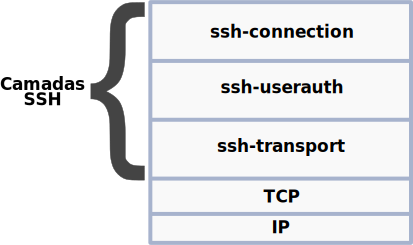
\includegraphics[width=0.4\textwidth]{ssh_layers}
  \caption{Camadas SSH \citep{opensshhood}}
  \label{fig:openssh_layer}
\end{figure}

Dado a enorme importância do OpenSSH, esse passa a ser alvo de constantes atques e também de aprimoramentos. Como resultado, algumas CVEs foram criadas e resolvidas no OpenSSH. Dentre as CVEs destacamos:


Do ponto de vista do uso de tal aplicação para validar propostas de abstrações de processos, destacamos que essa pode ser usada para demonstrar ganhos de segurança e controle de acesso a memória. Uma abordagem é partir de uma versão antiga do OpenSSH que não tem a correção para alguma vulnerabilidade e demonstrar que essa consegue resolver o problema. Note que os pontos mais fracos do OpenSSH podem ser destacados:

\begin{itemize}
  \item Acesso a chave é uma região crítica e que deve ter o seu acesso restrito;
  \item Potêncial vazamento de dados
  \item Escalada de privilégios
\end{itemize}
